% This is all preamble stuff that you don't have to worry about.
% Head down to where it says "Start here"
% --------------------------------------------------------------
 
\documentclass[12pt]{article}
\usepackage{tikz}
\usepackage[margin=1in]{geometry} 
\usepackage{amsmath,amsthm,amssymb}
\usepackage[margin=1in]{geometry} 
\usepackage{amsmath,amsthm,amssymb}
\usepackage[spanish]{babel} %Castellanizacion
\usepackage[T1]{fontenc} %escribe lo del teclado
\usepackage[utf8]{inputenc} %Reconoce algunos simbolos
\usepackage{lmodern} %optimiza algunas fuentes
\usepackage{graphicx}
\usepackage{setspace}
\usepackage{hyperref}
\usepackage{siunitx}
\usepackage{pgfplotstable}
\usepackage{pgfplots}
\usepackage{multicol}
\usepackage{lscape}
\usepackage{wrapfig}
\usepackage{tabularx}
\usepackage{caption}
\usepackage{booktabs}
\usepackage{fancyhdr}
\usepackage{subcaption}
\newcommand\mybar{\kern2pt\rule[-2pt]{.8pt}{11pt}\kern5pt}
\usepgfplotslibrary{external}
\tikzexternalize
\graphicspath{ {images/} }
\usepackage{hyperref} % Uso de links
\usepackage{lipsum}
 \newcolumntype{P}[1]{>{\centering\arraybackslash}p{#1}}
\newcommand{\N}{\mathbb{N}}
\newcommand{\Z}{\mathbb{Z}}
\sisetup{output-decimal-marker = {,}}
\sisetup{locale = DE}

\pgfplotsset{compat=1.14}


\begin{document}

 
% --------------------------------------------------------------
%                         Start here
% --------------------------------------------------------------
 \iffalse

\maketitle
\medskip
\fi

\begin{titlepage}
    \begin{center}
        \vspace*{1cm}
 
        \Huge
        \textbf{Entrega 2: Diagramas UML}
 
        \vspace{0.5cm}
        \LARGE
        PADSOF
 
        \vspace{1.5cm}
 
        \Large
        Grupo 5\\
        David del Val,\\
        Junco de las Heras,\\
        Jorge Fernandez
         
 
        \vfill
 
 
        \vspace{0.8cm}
 
 
        \Large
        Doble grado Informatica-Matematicas\\
        Grupo 2201\\
        UAM, Marzo 2020
 
    \end{center}
\end{titlepage}


\section{Diagrama de clases}

\begin{figure}[h!]
    \centering
    \includegraphics[scale=0.41]{Images/diagram_class.pdf}
    \vspace{+10pt}
\end{figure}
\newpage
El diagrama de clases es el primer diagrama que realizamos en esta fase del diseno ya que la definicion de las clases es necesaria para el resto de los diagramas
\par
El elemento central de nuestro diseno es la clase Aplicacion. Esta almacenara todas las instancias de las clases principales (\texttt{Usuario}, \texttt{Colectivo} y \texttt{Proyecto}). Respecto a la clase abstracta \textit{Usuario}, cabe destacar que la utilizamos para encapsular las clases \texttt{Ciudadano} y \texttt{Administrador} ya que estas comparten parte de su funcionalidad y atributos. 
\par
En segundo lugar, queremos comentar la relacion entre los colectivos y ciudadanos. Para el representate, hemos incluido una relacion de 1 a muchos mientras que los demas integrantes del colectivo se relacionan con este a través de la clase \textit{Elemento}. Esta nos permite expresar que tanto los ciudadanos como los colectivos (sub-colectivos) pueden formar parte de un colectivo. Entre \texttt{Colectivo} y \textit{Elemento} hemos establecido una relacion de agregacion ya que podemos considerar que los elementos estan contenidos en el colectivo.
\par
Por otra parte, la interfaz \textit{Elemento} se relaciona con \texttt{Proyecto} mediante dos tipos de asociaciones. En primer lugar, hemos de representar que un elemento (colectivo o ciudadano) puede apoyar a una serie de proyectos. Para ello, hemos utilizado una asociacion de muchos a muchos.
En segundo lugar, un colectivo o ciudadano puede proponer varios proyectos. Como un proyecto solo puede estar propuesto por una entidad, esta relacion es uno a muchos. 
\par 

Para representar los proyectos decidimos implementar una clase abstracta \textit{Proyecto} que contenga los atributos y la funcionalidad comun a todos los proyectos mientras que las particularidades de cada tipo se implementan en la clase correspondiente (\texttt{ProySocial} o \texttt{ProyInfraestructura}).
\par
Ya que los ciudadanos pueden subscribirse a proyectos para que se les informe de los cambios en el estado de estos, hemos creado una clase \texttt{Notificacion}. Cada ciudadano tendra sus propias notificaciones que se crearan cuando se produzcan cambios en proyectos que tengan al ciudadano en la lista de subscriptores

\par Por ultimo, queremos senalar que los distritos se han implementado con una clase en vez de una enumaracion para premitir anadir nuevos distritos durante el ciclo de vida de la aplicacion. En la fase de captura de requisitos, decidimos que al crear un proyecto de infraestructura, los distritos a los que afecta se eligirian de una lista de todos los distritos de la ciudad. Esta lista la hemos incluido en la clase aplicacion con la relacion de contenido.


\newpage
\section{Diagrama de transicion de estados de \texttt{Proyecto}}

\begin{figure}[h!]
    \centering
    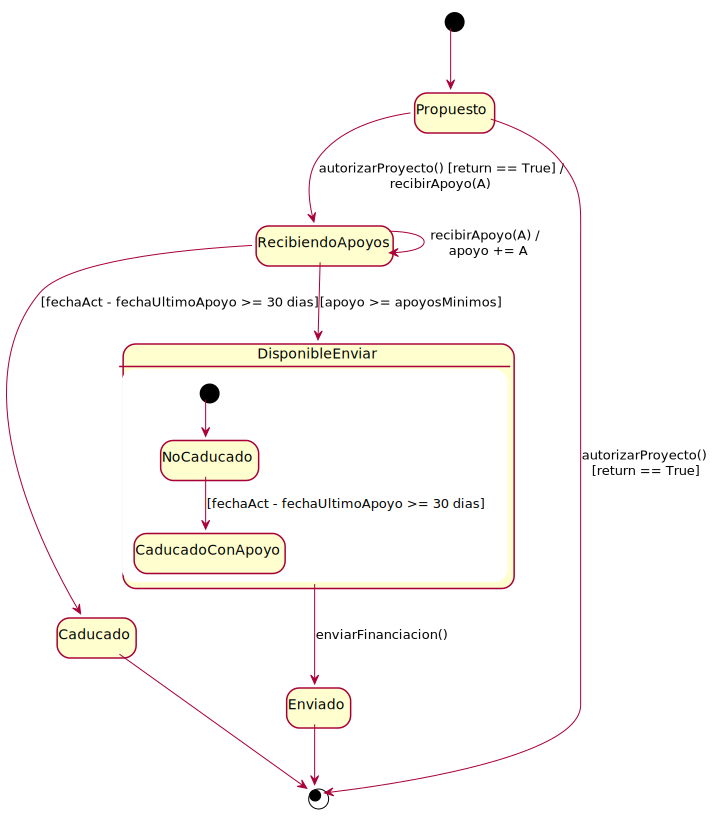
\includegraphics[scale=0.45]{Images/diagrama_estado_proyecto.pdf}
    \vspace{+10pt}
\end{figure}

Nuestro primer diagrama de transicion de estados describe la clase \texttt{Proyecto}. Elegimos esta clase ya que sus objetos son probablemente los que atraviesan mas estados.
\par
Al crear el proyecto este empieza en el estado de propuesto. En este estado, espera la accion del adminstrador, que tiene dos opciones, o deniega el proyecto (caso en el que el diagrama acaba) o lo acepta, pasando al estado de `RecibiendoApoyos'. En este permanece hasta que caduca (han pasado al menos 30 dias desde que recibio el ultimo apoyo) o llega al numero minimo de apoyos que necesita (apoyosMinimos) para poder ser enviado. 
\par 
En este ultimo caso entra en el estado jerarquico `DisponibleEnviar'. Este es el estado desde el que un proyecto puede ser enviado. Dentro de él, el objeto empieza como no caducado, pero pasa a `CaducadoConApoyo' si pasan 30 dias desde el ultimo apoyo. Esté caducado o no, si ya ha recibido el numero minimo de apoyos, este proyecto puede ser enviado al sistema externo.  

\newpage
\section{Diagrama de transicion de estados de \texttt{Ciudadano}}

\begin{figure}[h!]
    \centering
    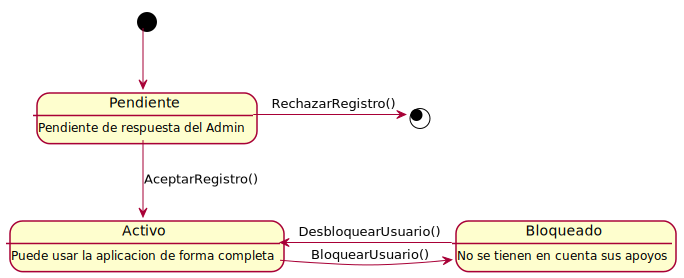
\includegraphics[scale=0.45]{Images/ciudadano_state.pdf}
    \vspace{+10pt}
\end{figure}
En el caso de la clase \texttt{Ciudadano}, sus instancias se crean cuando un individuo se registra en la aplicacion. Al registrarse, se le solicitan los datos necesarios para crear un nuevo usuario y este pasara al estado de `Pendiente'. Permanecera en este estado hasta que el administrador se pronuncie sobre el registro. Si el administrador rechaza el registro, el objeto pasara a un estado final de eliminado ya que esa instancia de \texttt{Ciudadano} ya no es necesaria.
\par
 
Por otra parte, si el administrador decide aprobar el registro, el usuario pasa a estar activo. Este es el estado en el que se prevé que el objeto esté durante la mayor parte del tiempo. Desde este estado, el administrador puede bloquear al ciudadano, lo cual lo pasaria al estado de `Bloqueado', donde sus apoyos ya no se tienen en cuenta. Del mismo modo, el administrador puede devolver al usuario al estado de activo.



\newpage
\section{Diagrama de secuencia de \texttt{crearProyectoColectivo}}

\begin{figure}[h!]
    \centering
    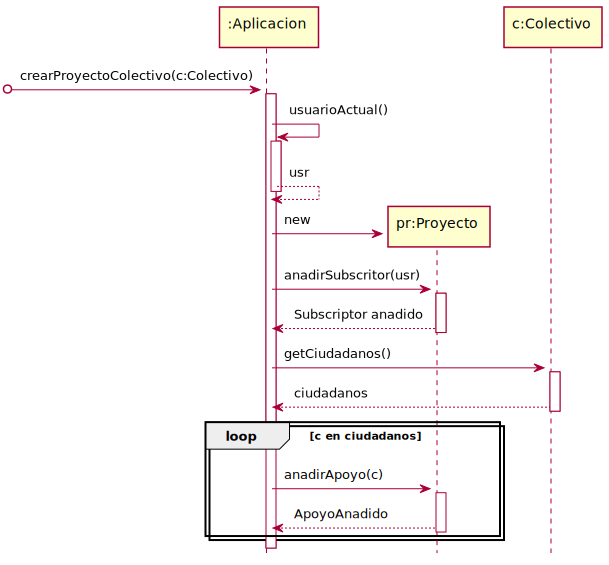
\includegraphics[scale=0.45]{Images/sequence_proyecto.pdf}
    \vspace{+10pt}
\end{figure}

La situacion que vamos a estudiar es la creacion de un nuevo proyecto por parte de un colectivo. Esta comienza con una peticion a la aplicacion en la que se indica el colectivo que esta solicitando la creacion del nuevo proyecto. 
\par
En primer lugar, la aplicacion solicita el usuario actual (que es el representante del colectivo) ya que este quedara subscrito al proyecto al haber sido el creador. Tras subscribir al usuario, la aplicacion obtiene la lista de ciudadanos que pertencen al colectivo \texttt{c} dado. Todos ellos deben de apoyar al proyecto ya que este esta siendo creado en nombre del colectivo. Por tanto, la aplicacion recorre la lista de ciudadanos y anade sus apoyos al Proyecto.

\newpage
\section{Diagrama de secuencia de \texttt{enviarProyecto}}
\begin{figure}[h!]
    \centering
    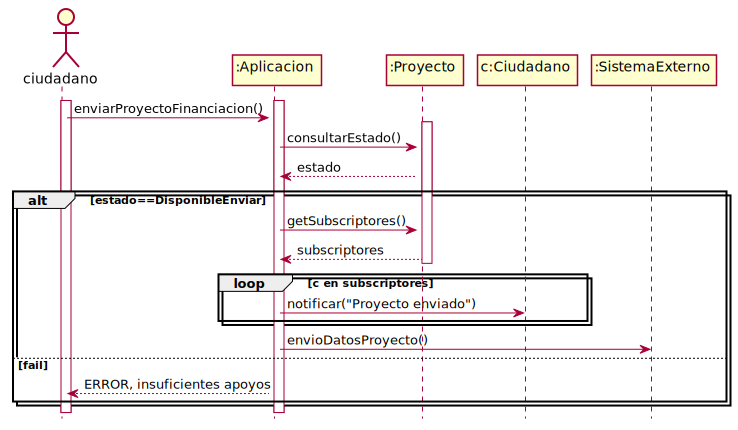
\includegraphics[scale=0.45]{Images/sequence_enviar_proyecto.pdf}
    \vspace{+10pt}
\end{figure}
En este ultimo diagrama vamos a analizar el escenario en el que un ciudadano envia un proyecto al sistema externo de financiacion. En primer lugar,el ciudadano envia una peticion de enviar proyecto a financiacion a la aplicacion, la cual consulta el estado del proyecto.
\par
Si su estado no es el de `DisponibleEnviar', la aplicacion devuelve un mensaje de error al usuario. Si, por el contrario, el proyecto puede ser enviado, se solicita la lista de los subscriptores. Esta esta compuesta por la persona que propuso el proyecto (o el representante del colectivo en su defecto) y los ciudadanos que se subscribieron individualmente. A cada uno de los ciudadanos en esta lista se les envia una notificacion de que el proyecto ha sido enviado y, finalmente, los datos del proyecto son entregados al sistema externo. 

\end{document}

